\documentclass[conference]{IEEEtran}


\usepackage{amsthm}
\usepackage[cmex10]{amsmath}
\usepackage{amsfonts}
\usepackage{amssymb}

\ifCLASSINFOpdf
\usepackage[pdftex]{graphicx}
\usepackage{subfigure}
\else

\usepackage{graphicx}
\usepackage{subfigure}
\fi
\usepackage{epstopdf}
\usepackage{color,xcolor}
%\usepackage[justification=centering]{caption}

\usepackage[font=normalsize]{caption}

\usepackage{algorithmic,algorithm}
\renewcommand{\algorithmicrequire}{\textbf{Input:}}
\renewcommand{\algorithmicensure}{\textbf{Output:}}
\newtheorem{theorem}{Theorem}
\newtheorem{lemma}{Lemma}
\newtheorem{remark}{Remark}
\newtheorem{proposition}{Proposition}
\newtheorem{corollary}{Corollary}
\renewcommand{\algorithmicrequire}{\textbf{Input:}}
\renewcommand{\algorithmicensure}{\textbf{Output:}}


\usepackage[numbers,sort&compress]{natbib}
\usepackage{color}
\renewcommand{\bibfont}{\footnotesize}

%\usepackage{hyperref}
%\usepackage{hypernat}

%\usepackage{cite}
%\usepackage{hyperref}
\usepackage{url}


\usepackage{mdwtab}

% correct bad hyphenation here
\hyphenation{op-tical net-works semi-conduc-tor equili-brium theo-retical calcula-ting func-tions}



\begin{document}
	
	\title{FlowCGAN: Exploratory Study of Class Imbalance for Encrypted Traffic Classification Using CGAN}
	
	
	% author names and affiliations
	% use a multiple column layout for up to three different
	% affiliations
	
	
\author{\IEEEauthorblockN{Pan Wang\IEEEauthorrefmark{1}, Shuhang Li\IEEEauthorrefmark{1}, Feng Ye\IEEEauthorrefmark{2}, 
		Zixuan Wang\IEEEauthorrefmark{1} and Moxuan Zhang\IEEEauthorrefmark{3}}
		\IEEEauthorblockA{
		\IEEEauthorrefmark{1}School of Modern Posts, Nanjing University of Posts \& Telecommunications, Nanjing, China\\
		\IEEEauthorrefmark{2}Department of Electrical \& Computer Engineering, University of Dayton, Dayton, OH, USA\\
		\IEEEauthorrefmark{3}Schools of International Education, Jinling Institute of Technology, Nanjing, China\\
		Email: \IEEEauthorrefmark{1}wangpan@njupt.edu.cn,
		\IEEEauthorrefmark{1}lish@runtrend.com.cn,
		\IEEEauthorrefmark{2}fye001@udayton.edu,
		\IEEEauthorrefmark{1}wangzx@runtrend.com.cn},
		\IEEEauthorrefmark{3}zhangmoxuan\_7@126.com}	
\maketitle
	
%Abstract	
\begin{abstract}
With more and more adoption of Deep Learning (DL) in the field of image proessing, computer vision and NLP, researchers have begun to apply DL to tackling with  encrypted traffic classification problems. Although these methods can automatically extract traffic features to overcome the difficulty of traditional classification methods like DPI in terms of feature engineering, a large amount of data is needed to learn the characteristics of various types of traffic. Therefore, the performance of classification model always significantly depends on the quality of datasets. Nonetheless, the building of datasets is a time-consuming and costly task, especially encrypted traffic data. Apparently, it is often more difficult to collect a large amount of traffic samples of those unpopular encrypted applications than well-known ones, which leads to the problem of class imbalance between major and minor encrypted applications in datasets. In this paper, we proposed a novel traffic data augmentation method called FlowCGAN using Conditional GAN, one of a genre of Generative Adversarial Network (GAN) . As a generative model, FlowCGAN exploit the benefit of GAN {\color{red} and CGAN's benefit?} to generate new traffic samples by learning the characteristics of the traffic data and thereby balancing between major and minor classes of the datasets. As a proof of concept, Convolutional Neural Network (CNN) was adopted and designed to classify three encrypted traffic datasets: the original unbalanced dataset, the dataset augmented by Random Over Sampling (ROS) method and the new augmented dataset based on FlowCGAN respectively. The experimental evaluation results demonstrate that CNN based encrypted traffic classifier over our new dataset based on FlowCGAN can achieve better performance than the other two in terms of encrypted traffic classification.
\end{abstract}

\begin{IEEEkeywords}
encrypted traffic classification, data augmentation, Conditional Generative Adversarial Network, traffic identification, class imbalance
\end{IEEEkeywords}


% Introduction
\section{Introduction}\label{sec:intro} % add a label for reference
With the rapid development of network technology, the types and quantity of traffic data in cyberspace are increasing. Network traffic identification and classification is a crucial research task in the area of network management and security. It is the footstone of dynamic access control, network resources scheduling, content based billing, intrusion and malware detection etc. High efficient and accurate traffic classification is of great practical significance to provide service quality assurance, dynamic access control and abnormal network behaviors detection. With the widespread adoption of encryption techniques for internet, especially 5G and IoT applications, the growth of portion of encrypted traffic has dramatically posed a huge challenge for QoS, network management and security monitoring. Therefore, studies on encrypted traffic classification not only help to improve the fine-grained network resource allocation based on application, but also enhance security level of network and applications.


Traditionally, the evolution of encrypted traffic classification technology has gone through three stages: port matching, payload matching and flow statistical characteristics based classification methods. Port matching based method infers applications' types by assuming that most applications consistently use 'well known' TCP or UDP port numbers, however, the emergence of port camouflage, dynamic port, proprietary protocols with user-defined ports and tunneling technology makes these methods lose efficacy quickly. Payload matching based methods, namely, DPI (Deep Packet Inspection) technology cannot deal with encrypted traffic because of invisible packet content of encrypted traffic, in addition, it incurs high computational overhead and requires manual signatures maintenance~\cite{Finsterbusch2014,SDN-HGU,PhoneNumber}. As a result, in order to attempt to solve the aboved problems of encrypted traffic identification , flow-based methods emerged, which usually combine statistical or time series traffic features with Machine Learning (ML) algorithms,  such as naive bayes(NB), support vector machine(SVM), decision tree, Random Forest(RF), k-nearest neighbor(KNN) ~\cite{Pescape2008,Sun2010,Velan2015,Arndt2011}. Although classical machine learning approaches can solve many issues that port and payload based methods cannot solve, it still has some limitations, such as handcrafted traffic features driven by domain-expert, time-consuming, lack of ability of automation, rapidly outdated when compared to the evolution. Unlike most traditional ML algorithms, DL performs automatic feature extraction without human intervention, which undoubtedly makes it a highly desirable approach for traffic classification, especially encrypted traffic.  Recent research work has demonstrated the superiority of DL methods in traffic classification~\cite{MobileTC-2018}, such as MLP~\cite{Datanet}, CNN~\cite{deeppacket,Wang-1D-CNN,Wang2D-CNN,Seq2Img,HierarchicalTC}, SAE~\cite{blackhat}, LSTM~\cite{IoT-CNN-2017,HAST-IDS}. 





However, due to the different popularity of various applications, the class imbalance problem of traffic samples often occurs when building traffic datasets. That is, the number of popular applications samples is much larger than others, which always leads to the misclassifying problems of minor applications and thereby incurs deterioration of classifier performance. Imbalanced class distribution of a dataset has posed a serious challenge to most ML based classifiers which assume a relatively balanced distribution~\cite{Japkowicz:2002}. Network traffic classification is no exception due to the imbalanced property of network traffic data~\cite{Vu2017,Vu2016}, especially encrypted traffic. Therefore, it is very crucial to address such challenges of imbalanced class distribution of traffic datasets for network traffic classification. However, there are very few studies focusing on traffic data augmentation for traffic classification to overcome the limitation of class imbalance.

In this paper, we proposed traffic data augmentation method called FlowCGAN using Conditional GAN, one of a genre of GAN. As a generative model, FlowCGAN exploits the benefit of GAN to generate synthesized traffic samples by learning the characteristics of the original traffic data. The synthesized data is then combined with the original (viz. real) data to build the new traffic dataset and thereby keep balance between major and minor classes of the dataset. As a proof of concept, CNN was adopted and designed to classify three encrypted traffic datasets: the original unbalanced dataset, the dataset based on ROS~\cite{ROS2004} method and the new augmented dataset based on FlowCGAN respectively. The experimental evaluation results show that classical deep learning based encrypted traffic classifier over our new dataset based on FlowCGAN method can achieve better performance than the other two in terms of encrypted traffic classification.


{\color{red} need to modify:} The rest of this paper is organized as follows. Section II introduces the preliminaries and related works of traffic classification, some current methods for tackling with the problem of imbalanced class data and GAN. Section III illustrates the algorithm of FlowCGAN. Section IV describes the design of the encrypted traffic classification method based on FlowGAN. The experimental results are provided and discussed in Section V. Section VI  concludes our work and presents some future works.


\section{Related works}\label{sec:related_works}
\subsection{ML and DL based approach of Traffic Classification}
Different from port and payload matching methods, ML based classification methods always use payload-independant parameters such as packet length, inter-arrival time and flow duration to circumvent the problems of encrypted content and user's privacy~\cite{2007legal}. Many work was carried out using ML algorithms during the last decades. In general, there are two learning strategies used: one is the supervised methods like decision tree, SVM and Naive Bayes, the other is unsupervised approaches like k-means and PCA~\cite{2008NguyenTC}. Nevertheless,  many drawbacks hindered ML based methods widely applied to traffic classification, such as handcrafted traffic features driven by domain-expert, time-consuming, unsuited to automation, rapidly outdated when compared to the evolution. Unlike most traditional ML algorithms, Deep Learning performs automatic feature extraction without human intervention, which undoubtedly makes it a highly desirable approach for traffic classification, especially encrypted traffic.  Recent research work has demonstrated the superiority of DL methods in traffic classification~\cite{MobileTC-2018,deeppacket,Datanet,Wang-1D-CNN,Wang2D-CNN,IoT-CNN-2017,HAST-IDS,Seq2Img,blackhat,TC-VAE,HierarchicalTC}. The workflow of DL based classfication usually consists of three steps. First, model inputs are defined and designed according to some principles, such as raw packets, PCAP files or flow statistics features. Second, models and algorithms are elaborately chosen according to models' characteristics and aim of the classifier. Finally, the DL classifier is trained to automatically extract the features of traffic.

\subsection{Traditional methods for handling imbalanced data}
In general, there are three methods for dealing with class imbalance problem: \emph{\textbf{Modifying the objective cost function, Sampling and Generating artificial data}}~\cite{Vu2016}. The approach of \emph{\textbf{modifying objective cost function}} alleviates the problem by means of weighting differently the data samples in minor and major classes, which gives higher score on the minor samples to penalize more intensely on miss-classifiying of the sample in the minor class. Sampling methods include two different ways of \emph{\textbf{under-sampling}} and \emph{\textbf{over-sampling}}, which is to reduce the size of major class by removing some major data samples and raise the ones in the minor class, respectively. Random under sampling (RUS) and Random over sampling (ROS) are two main methods of under-sampling and over-sampling~\cite{ROS2000}. RUS randomly removes some instances in major class, accordingly, ROS generates some copies of samples of the minor class. However, overfitting problem is always the main drawback of ROS due to generating same copies from the minor class. A classical method for generating artificial data is Synthetic Minority Over-sampling Techinique (SMOTE) in which minority samples are generated by synthetic samples rather than copies~\cite{SMOTE2002}.

\subsection{The application of GAN and other DL techniques in generating traffic data samples}
Due to the great success of GAN applying in images, computer vision and NLP etc., this innovative technique has been already applied to network security recently. A few current studies have shown that GAN has been applied in IDS and Malware detection to generate adversarial attacks to deceive and evade the detection systems~\cite{Lin2018IDSGANGA,Hu2017GAN} and thus effectively improve the performance of malware detection or IDS~\cite{Hu2017GAN,KimGAN,Lin2018IDSGANGA,Salem2018GAN,Knife-Fight}. Correspondingly, as for traffic classification, some researchers have introduced some approaches based on GAN to generate the traffic samples to overcome the imbalaced limitation of network data. In~\cite{Vu-GAN}, the authors proposed a novel method called auxiliary classifier GAN (AC-GAN) to generate synthesized traffic samples for balancing between the minor and major classes over a well-known traffic dataset NIMS. The AC-GAN took both a random noise and a class label as input in order to generate the samples of the input class label accordingly. The experimental results has shown that their proposed method achieved better performance compared to other methods like SMOTE. However, the NIMS dataset was only composed of  SSH and non-SSH two classes. In ~\cite{Hasibi2019AugmentationSF}, the authors proposed a novel data augmentation approach based on the use of Long Short Term Memory (LSTM) network to learn the traffic flow patterns and Kernel Density Estimation (KDE) for replicating the sequence of packets in a flow for classes with less population. The results have shown that this method can improve the performance of DL algorithms over augmented datasets. {\color{red} need to add some description of the drawback of ACGAN and LSTM methods.}

\section{Generative Adversarial Networks}\label{gan}
\subsection{GAN}\label{AA}
As an unsupervised learning model, a classic GAN network consists of two parts, the generator $G$ and the discriminator $D$. %As shown in Fig.~\ref{fig_gan},% 
The role of the generator is to take random noise as input by learning the characteristic distribution of real data. The discriminator aims at determining whether the data is real or generated by $G$.  
The generator $G$ simulates the feature distribution $P_g$ of the real data by the prior distribution $P_z(z)$. The input of the discriminator is the real and generated data, correspondingly, the output $D(x)$ indicates the probability of whether the input data is real or not~\cite{r11}. During the training process, $G$ and $D$ play a two-player mini-max game until $D$ can't judge whether the sample data is real, which means that the two networks reach the Nash Equilibrium. The objective function of GAN can be expressed by \eqref{GAN}:
\begin{equation}
\begin{split}
\label{GAN}
\mathop {\min }\limits_{\rm{G}} \mathop {\max }\limits_D V(D,G) = \mathbb{E}_{x\sim{p_{data}}(x)}[\log D(x)] \\
+ {\mathbb{E}_{z\sim{p_z}(z)}}[\log (1 - D(G(z)))]
\end{split}
\end{equation}

\iffalse
\begin{figure}[htbp]
	\centerline{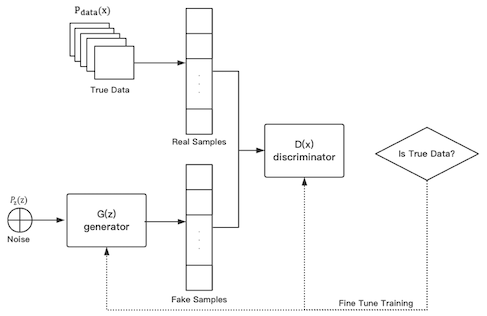
\includegraphics{fig/GAN-20191017.png}}
	\caption{Network structure of GAN.}
	\label{fig_gan}
\end{figure}
\fi 



In Equation \eqref{GAN}, $P_{data}(x)$ represents distribution of the real data. When training $D$, the goal is to optimize the probability of TRUE $D(G(z))$ as small as possible and the probability of TRUE $D\left(x\right)$ of the real data $x$ as much as possible. When training $G$, the goal is to make $D(G(z))$ as much as possible. From \eqref{GAN}, we can calculate the optimal discriminator as \eqref{eq1}. As can be seen from \eqref{eq1} below, when $P_{data}\left(x\right)=P_z\left(z\right)$, it means that $D$ cannot distinguish whether the sample is true or false, $D$ and $G$ reach the Nash Equilibrium, and the discriminator output is 0.5.

\begin{equation}
\begin{split}
\label{eq1}
%D^*(x)=\frac{P_{data}(x)}{P_{data}(x)+P_z(z)}
D(x)=\frac{P_{data}(x)}{P_{data}(x)+P_z(z)}
\end{split}
\end{equation}

\subsection{CGAN}
{\color{blue}In GAN, there is no control over modes of the data to be generated. The conditional GAN changes that by adding the constraint condition $y$ as an additional parameter to the generator $G$ and hopes that the corresponding images are generated. For example, in MNIST, the digit generated by GAN may be either any digit from 0-9 instead of specified one or always output the same digit. Fig.~\ref{fig_cgan} shows the network structure of CGAN.}


%When compared with other complex generative models, GAN's min-max competition makes it possible to generate data without pre-modeling. It only needs to learn the distribution of the real data and approximate them. This is the intrinsic characteristics of GAN, nevertheless, it also has the disadvantage that it is intractable to train the generative model steadily and thus incurs mode collapse.  In order to solve this problem, Montreal et al. proposed Conditional Generative Adversarial Nets (CGAN~\cite{r12}) to address such problems. The method guides the data generation process by adding a constraint condition y to both $D$ and $G$. This simple improvement has been effectively and widely used in many application scenarios.  %



\begin{figure}[htbp]
	\centerline{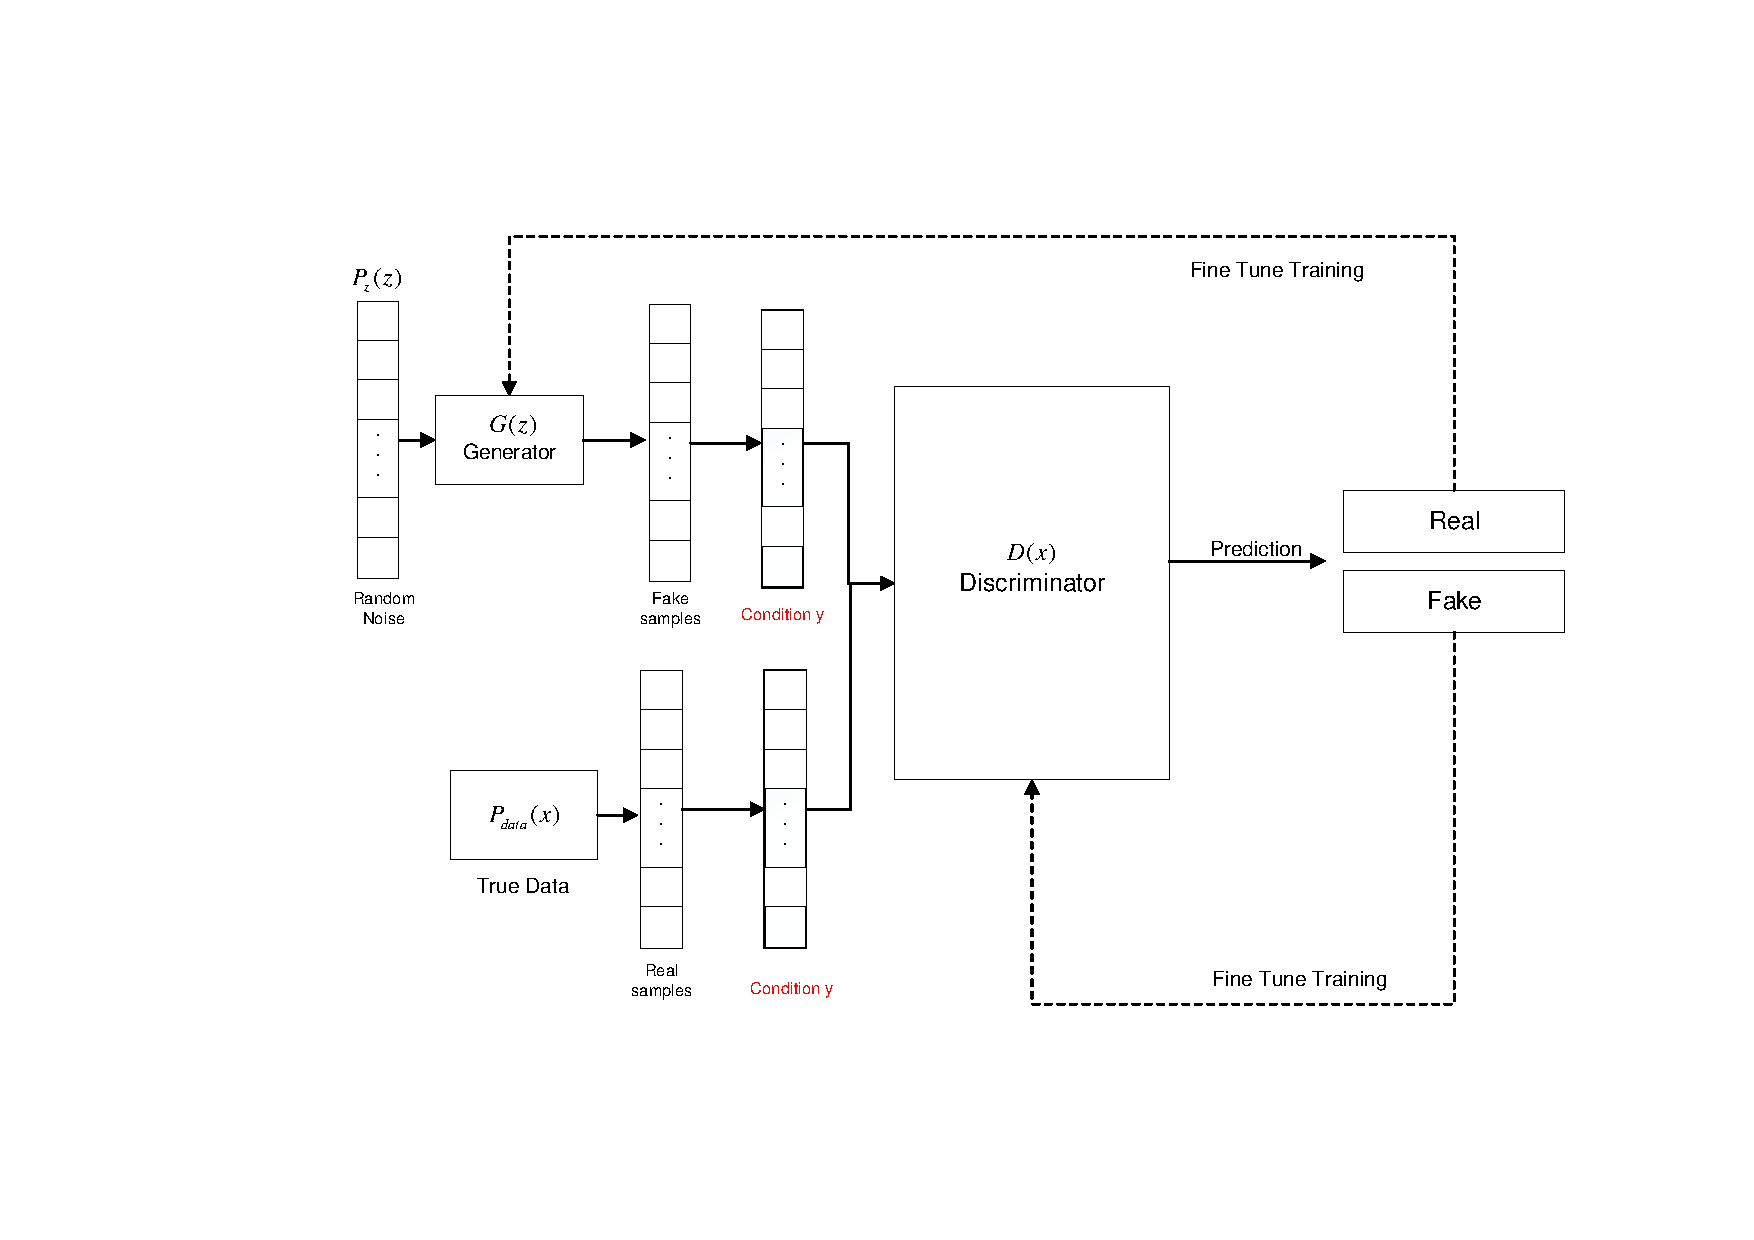
\includegraphics[width=8cm, height=6cm]{fig/CGAN-20191017.pdf}}
	\caption{The network structure of CGAN.}
	\label{fig_cgan}
\end{figure}

The principle, structure and training process of CGAN are similar to GAN. The cost function is slightly different as is shown in \eqref{CGAN}:

\begin{equation}
\begin{split}
\label{CGAN}
\mathop {\min }\limits_{\rm{G}} \mathop {\max }\limits_D V(D,G) = \mathbb{E}_{x\sim{p_{data}}(x)}[\log D(x|y)] \\
+ {\mathbb{E}_{z\sim{p_z}(z)}}[\log (1 - D(G(z|y)))]
\end{split}
\end{equation}

As shown in Fig.~\ref{fig_cgan}, CGAN's training process includes the following steps:
\begin{itemize}
	\item Sampling the real data to obtain $P_{data}(x)$, obtaining the label $y$ corresponding to the sampling data $P_{data}(x)$, feed $P_{data}(x)$ and $y$ into the discriminator $D$, then updating the parameters according to the output results;
	\item Generating random noise $P_z(z)$, which is then fed into generator $G$ together with label $y$ in the above step, and $G$ generates synthesized data.
	\item Feeding the synthesized data and the label $y$ generated in the above step into the discriminator $D$, and $G$ will optimize the parameters according to the output result of $D$.
	\item Repeat the above steps until $G$ and $D$ reach the Nash equilibrium.
\end{itemize}

\subsection{InfoGAN}
{\color{purple}In CGAN, the labels $y$ always explicitly are read and passed into the generator $G(z,y)$ and discriminator $D(x,y)$. However, in InfoGAN, the generator and discriminator are $G(z,c)$ and $D(x)$, which $c$ is the latent code representing the semantic features of the datapoints and the noise vector $z$ is the source of noise for the latent variables similar to CGAN. In InfoGAN, $c$ will be learned from $x$ in a DNN instead of initializing it explicitly with labels in CGAN. The codes are then made meaningful by maximizing the Mutual Information between the code and the Generator $G$ output. The objective function of the InfoGAN is as shown in Equation \eqref{InfoGAN}.  }

\begin{equation}
\begin{split}
\label{InfoGAN}
\mathop {\min }\limits_{\rm{G}} \mathop {\max }\limits_D V_I(D,G) = V(D,G)-\lambda I(c;G(z,c))
\end{split}
\end{equation}
with

\begin{equation}
\begin{split}
\label{V_InfoGAN}
V_{GAN}(D,G) = \mathbb{E}_{x\sim{p_{data}}(x)}[\log D(x)] \\
+ {\mathbb{E}_{z\sim{p_z}(z)}}[\log (1 - D(G(z,c)))]
\end{split}
\end{equation}

{\color{purple}To compute $I(c,G(z,c))$, it is necessary to approximate $p(c|x)$ with a function $Q(c|x)$(Variation Maximization), which is as follows:}

\begin{equation}
\begin{split}
\label{Variation_Maximization}
\mathbb{E}_{x\sim{G(z,c)},c\sim{p(c|x)}}[\log p(c|x)] \\
= \mathbb{E}_{x\sim{G(z,c)},c\sim{p(c|x)}}[\log Q(c,x)] + \\ \mathbb{E}_{x\sim{G(z,c)},c\sim{p(c|x)}}[\log \frac{p(c|x)}{Q(c,x)}] \\
=  \mathbb{E}_{x\sim{G(z,c)},c\sim{p(c|x)}}[\log Q(c,x)] + \\
\mathbb{E}_{x\sim{G(z,c)},c\sim{p(c|x)}}[{D_{KL}(p(c|x))}||{Q(c,x)}]\\
\geq  \mathbb{E}_{x\sim{G(z,c)},c\sim{p(c|x)}}[\log Q(c,x)] 
\end{split}
\end{equation}



% Reference
% Please update the Reference.bib
\renewcommand\refname{Reference}
\bibliographystyle{IEEEtran}
\bibliography{IEEEfull,Reference}


\end{document}


